\documentclass{article}
\usepackage{hyperref}
\usepackage{graphicx}
\hypersetup{
    colorlinks,
    citecolor=black,
    filecolor=black,
    linkcolor=black,
    urlcolor=black
}
\begin{document}
		\begin{figure}[t]
			\centering
			
\includegraphics[width=350px]{UP_Logo.PNG}
		\end{figure}
			\title{COS 301 Software Engineering -Architectural Requirements Specifications and Design for the NavUP System}
\maketitle
		\begin{center}
			\textbf{\newline Group Ruby} \\
		\end{center}
			
				
		\begin{flushright} \large
			Matthew Perry - u13017030 \\
			Unarine Rambani - u14004489  \\
			Phuti Setoaba -  u13032616\\
			Mankgwanyane Tlaka - u14351872  \\
			Victor Twigge -  \\
			Bernard van Tonder -  \\
		\end{flushright}
		
		
		
		
		GitHub Repository: \href{https://github.com/perrymatthew/cos301_team_ruby}\\
		\url{https://github.com/perrymatthew/cos301_team_ruby}
	

\clearpage
\tableofcontents

\clearpage
\section{Introduction}
	

\clearpage
\section{Requirements}
	\subsection{External Interface Requirements}
    \subsubsection{User Interface}
    
        \subsubsubsection{\textbf{Login Interface}}
            The user will be presented with a login form with a username/email and a password field. The password field will hide input in order to ensure security. An error message wil be displayed if the user inputs incorrect details for these fields. In the case that the user is not registered, a 'Register' option will be provided below the form; clicking on this link will present the user with a registration form.
    \\  \\
        \subsubsubsection{\textbf{Search Interface}}
            An interactive search bar will be persisted at the top of the device screen. A user can click on the search bar and enter the name of a location to search for it.
    \\  \\
        \subsubsubsection{\textbf{Navigation Interface}}
            Once a user's current and destination locations have been determined, the user will be required to press the 'Navigate' button in order to bring up the Navigation view that will render and display a view of the user's navigation session. 
    \\  \\
        \subsubsubsection{\textbf{Administration Control Panel Interface}}
            This interface will allow users with Administrator privileges to manage location and event information.
    \\  \\
    \subsubsection{Hardware Interface}
        For the mobile applications, the user will need to will need an Android or iOS mobile device. The web portal does not have any hardware interfaces since it will not be developed for specific operating systems. GPS functionality will be handled by the device's built-in GPS application and connectivity to the server would be managed by the underlying operating system.
        
    \subsubsection{Software Interface}
    The mobile application will communicate with the GPS application in order to acquire spatial data; the application will also communicate with the database server to get information about different locations that are available on campus. The system will need either an operating system or a web browser in order to be operable.
        
    \subsubsection{Communication Interface}
    Communication between the different parts of the system will be handled by the underlying operating system. Communication with the server will be done using the HTTP/HTTPS protocol over the device's internet/wifi connections

\subsection{Performance Requirements}
    \\ \\
    \subsubsubsection{\textbf{Search Feature}}
        The search feature should be prominent so that it is easily locatable for the user.
    \\ \\    
    \subsubsubsection{\textbf{Search Results}}
        Results from the search feature should be displayed in a list if more than one location is returned.
    \\ \\
    \subsubsubsection{\textbf{Response Times}}
        \begin{itemize}
            \item The mobile application and the web portal should be interactive and responsive.
            \item The system should respond to user input almost immediately.
            \item Searches must be completed within 2 seconds.
            \item Acquire the user's location with an accuracy within an 8m radius.
			\item Display the user's location on a map within 3 seconds after launching.
			\item Generate routes for users within 2 seconds.
			\item Update the user's location every second when navigating.
        \end{itemize}
    \\ \\
    \subsubsubsection{\textbf{Dependability}}
        \begin{itemize}
            \item The system should give the user an indication when executing a process that will require the user to wait.
            \item The system should display a message if an error is encountered.
        \end{itemize}

\section{Design constraints}
	\begin{itemize}
    \item User and location information will be stored in a database that will be accessible via the system.
    \item The system should \textbf{always} be available.
    \item Users will be able to access the system from any mobile device that has Internet browser capabilities or from Android/iOS mobile devices that have the application installed
    \item Users must be registered and logged-in with correct details in order to perform functions
    \item The application should not take up more than 10MB(Megabytes) of the devices' disk space
    \item The GIS module must be limited to the Hatfield campus only
    \item Guest user's Functionalties must be limited, for all user functionality they must be a registered user
    \item Admin must only add locations that do not exist in the systems- i.e locations should not be duplicated
    
\end{itemize}

\section{Software system attributes}
	\subsection{Reliability}
\begin{itemize}
    \item The system should generate accurate results for searches. A message should be displayed if a location cannot be found or the search cannot be performed.
    \item The system should determine user location and display level of accuracy for triangulation.  
    \item The system should generate correct and reasonable routes when provided with two locations.
    \item Users with administration privileges should be able to create, update and remove locations.
    \item Notifications should be sent to all registered users via email or SMS.
\end{itemize}

\subsection{Availability}
\begin{itemize}
    \item The system should always be available.
    \item An Internet connection should be available for the application to communicate with the database.
    \item The application should be connected to the built-in GPS application so that the user's location can be determined.
    \item Users should be notified if the system is not available.
    
\end{itemize}

\subsection{Security}
\begin{itemize}
    \item Communication between the application and the user database should be encrypted.
    \item If a user attempts to log in with invalid credentials, they should not be given access and a failure message should be displayed.
    \item Only users with administration privileges should be able to perform functions that deal with the management of location objects and events.
    
\end{itemize}

\subsection{Maintainability}
\begin{itemize}
    \item The system should be implemented with as little coupling as possible, so that it is easy to add new functions and extend it.
    \item Tests must be built for each module in isolation, in order to determine their functionality. 
\end{itemize}
\subsection{Portability}
    \begin{itemize}
        \item The application should be portable with both Android and iOS platforms.
    \end{itemize}
\clearpage

\section{Access Modules}
	\subsection{Use Case Diagram}
\begin{figure}[H]
	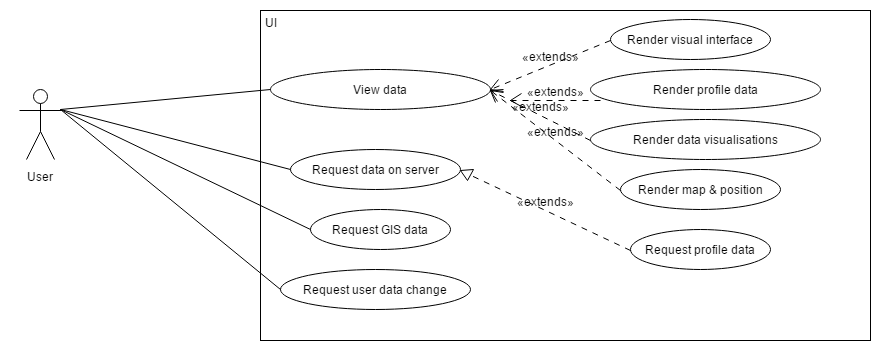
\includegraphics[width=\textwidth]{Access_Modules/AUCD_v2.png}
\end{figure}

\subsection{State Diagram}
\begin{figure}[H]
	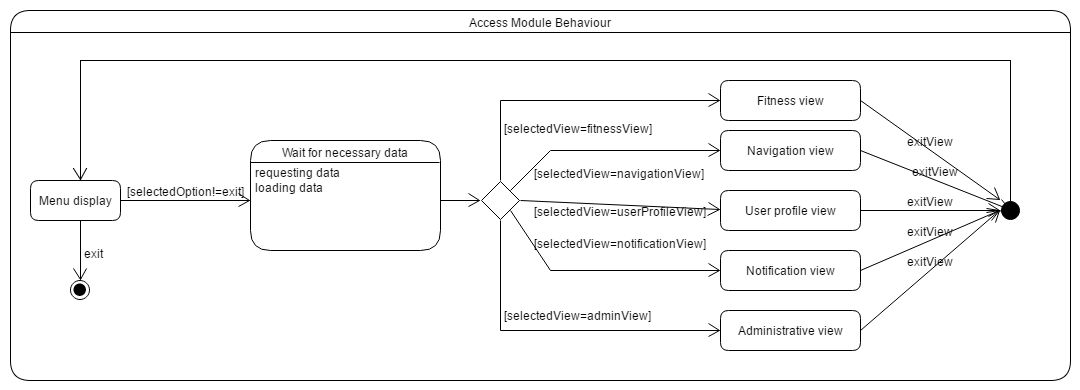
\includegraphics[width=\textwidth]{Access_Modules/AccessStateDiagram.png}
\end{figure}

%\subsection{Sequence Diagram}

%\subsection{Package Diagram}

\subsection{Activity Diagram}
\begin{figure}[H]
	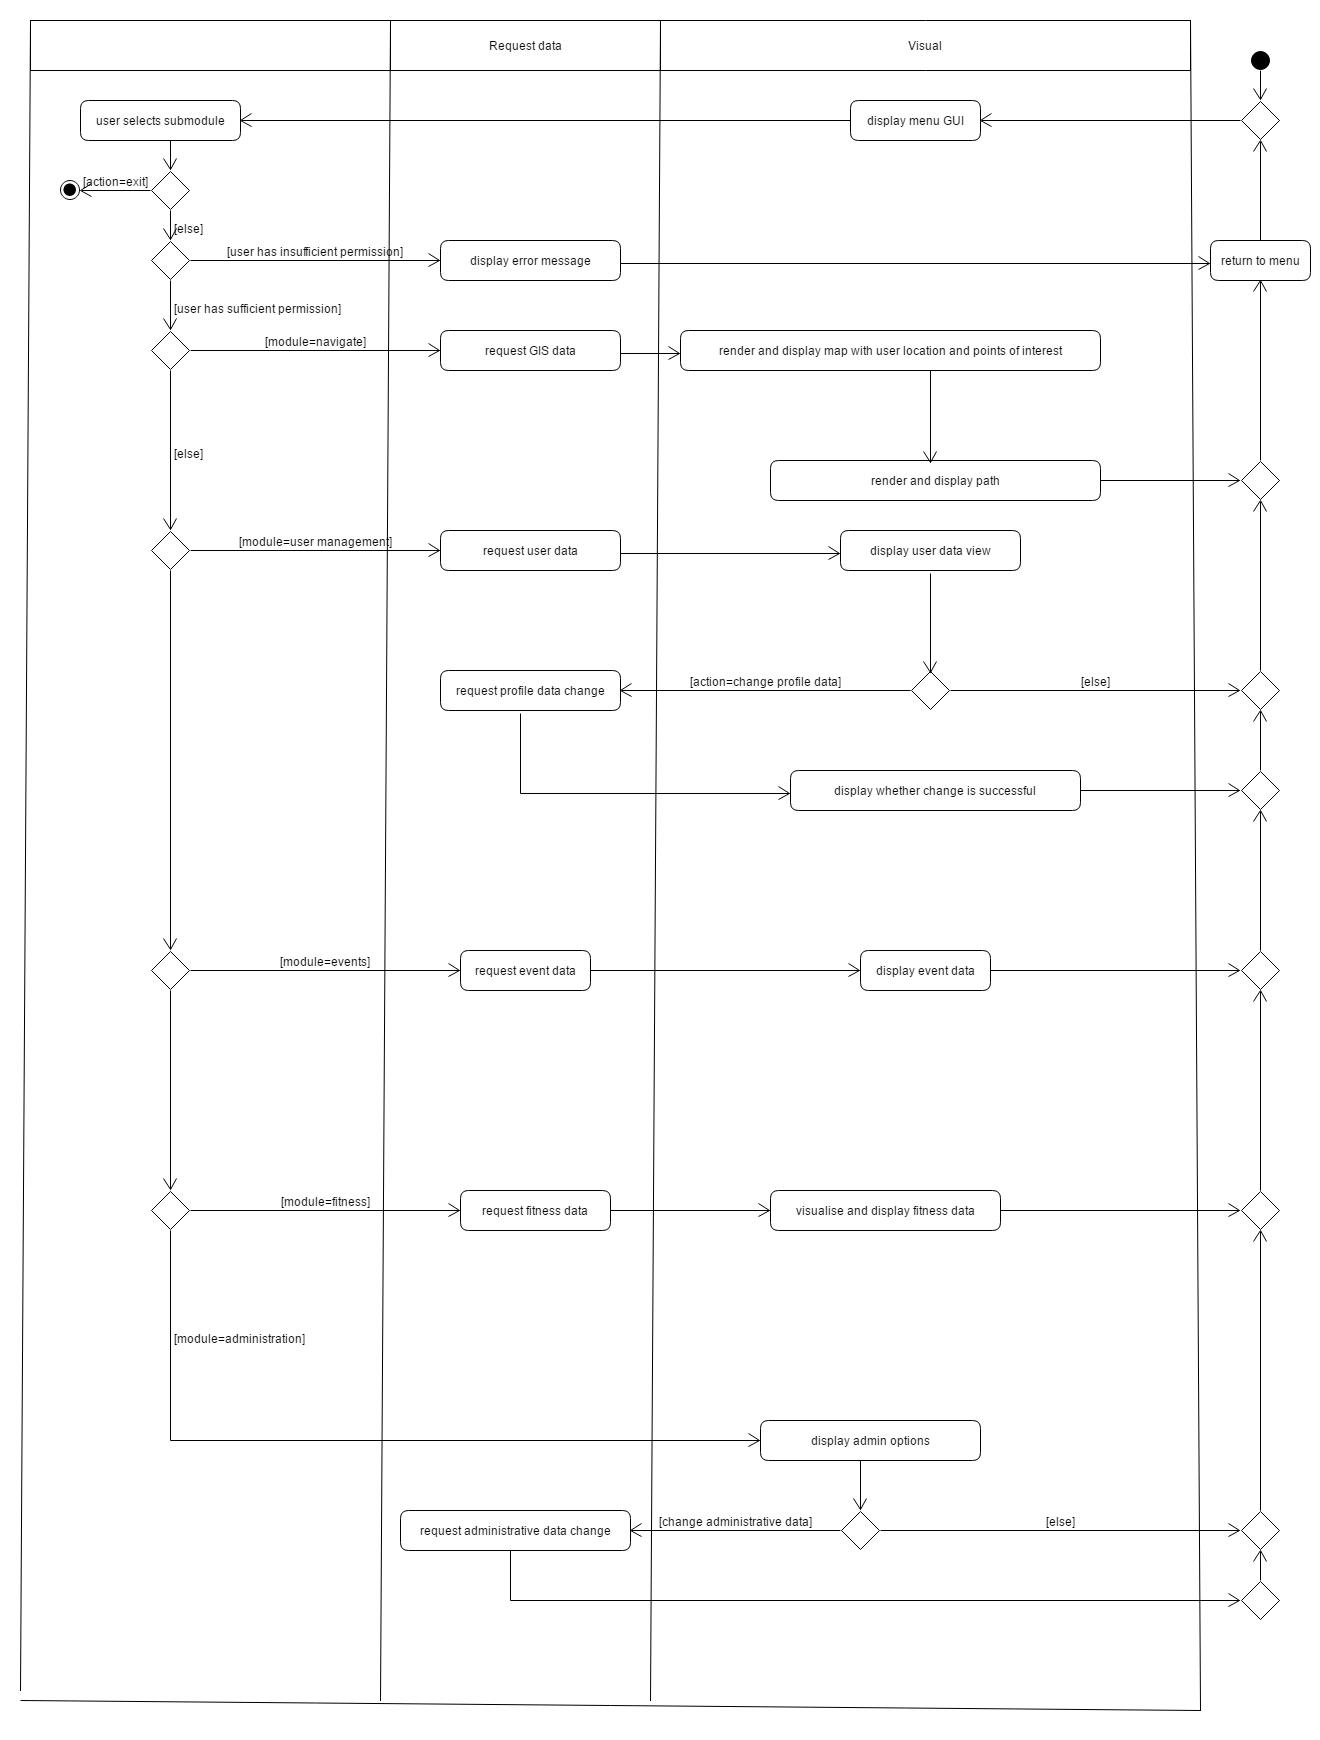
\includegraphics[width=\textwidth]{Access_Modules/AcessActivity.png}
\end{figure}

\subsection{Class Diagram}
\begin{figure}[H]
	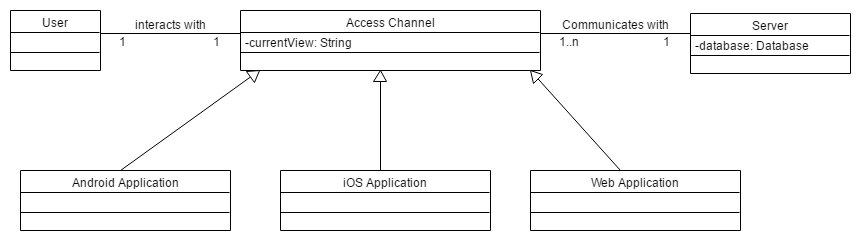
\includegraphics[width=0.8\textwidth]{Access_Modules/AccessClassDiagramV2.png}
\end{figure}

\clearpage

\section{GIS}
	\subsection{Use Case Diagram}

The GIS module Use Case requires an agent to be able to add GIS objects to the database. These objects contain both spacial data for their real life location, and attribute tables which contain the meta data about each object. \\
\begin{figure}[!h]
  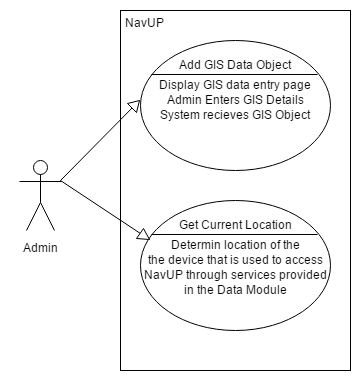
\includegraphics[width=0.6\textwidth]{GIS/GIS_Use_case.png}
\end{figure}

\subsection{State Diagram}
The GIS module is not a state dependant system.

\subsection{Sequence Diagram}

\subsection{Package Diagram}

\subsection{Activity Diagram}
\begin{figure}[!h]
	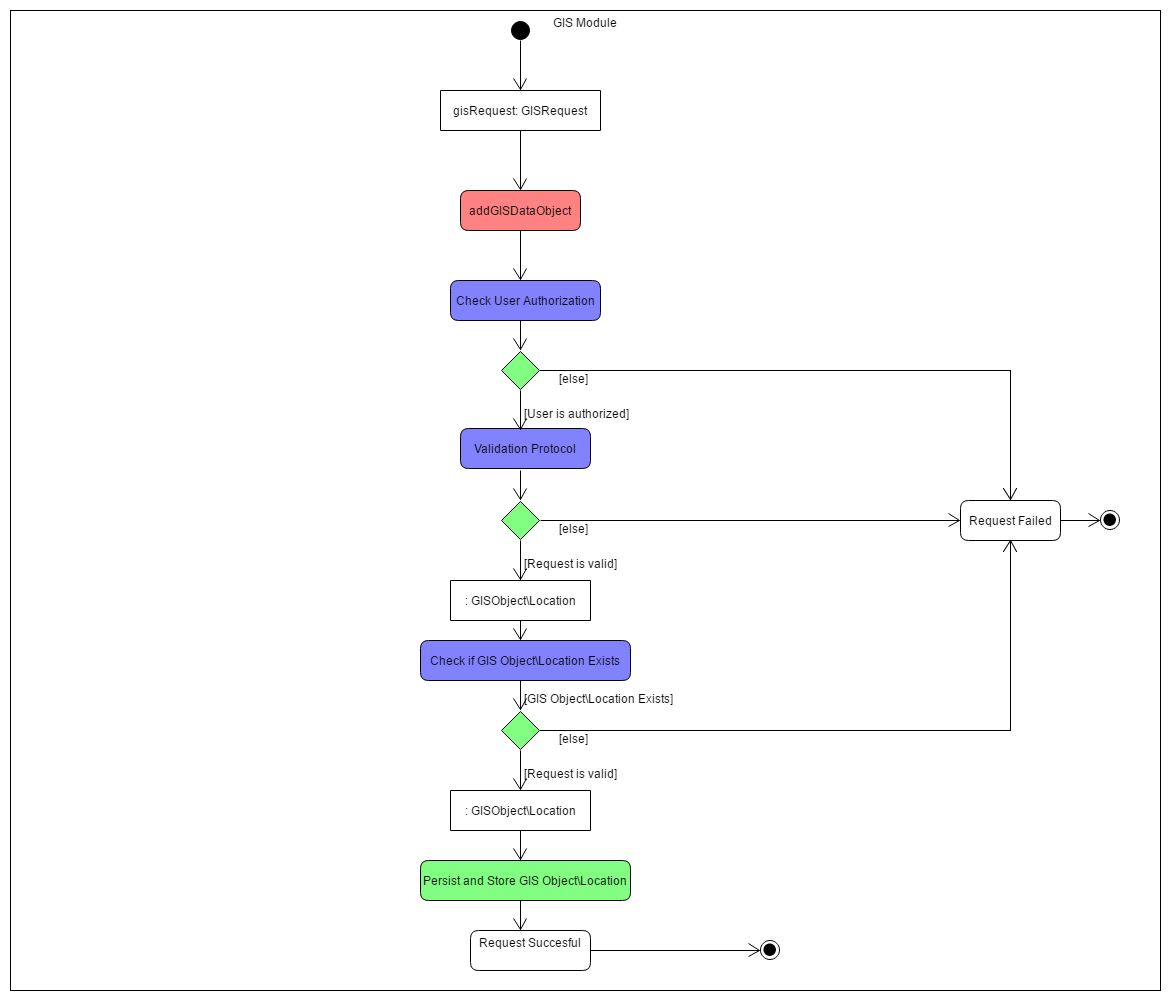
\includegraphics[width=\textwidth]{GIS/GIS_Activity-addGISObject.png}
\end{figure}

\subsection{Class Diagram}
\begin{figure}[!h]
	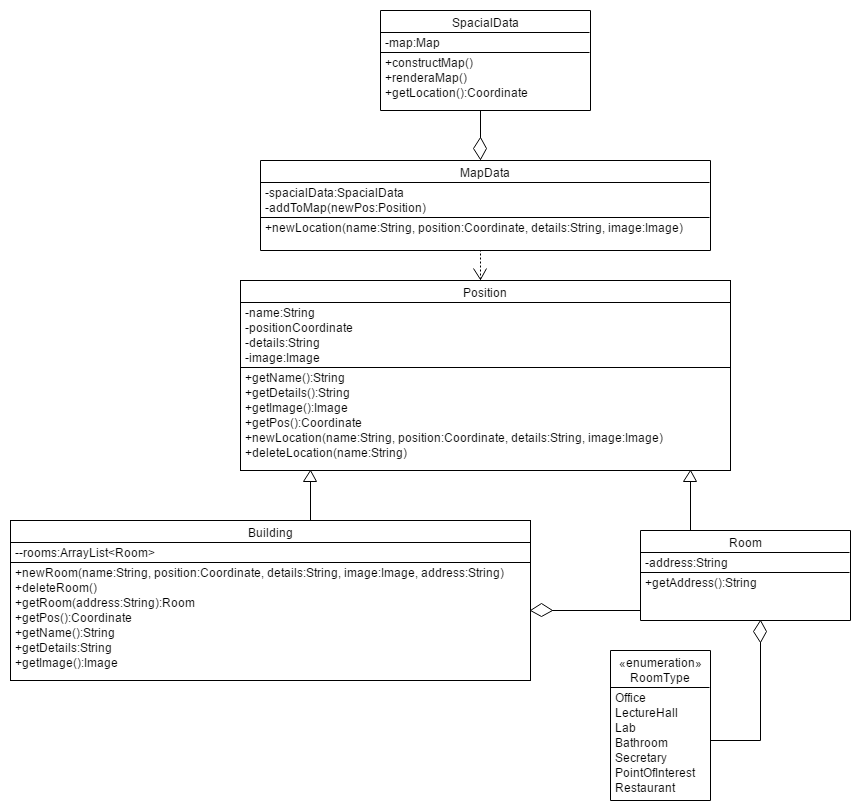
\includegraphics[width=\textwidth]{GIS/GIS_Class_Diagram.png}
\end{figure}
\clearpage

\section{User Management}
	\subsection{Use Case Diagram}

\subsection{State Diagram}
\begin{figure}[!htbp]
	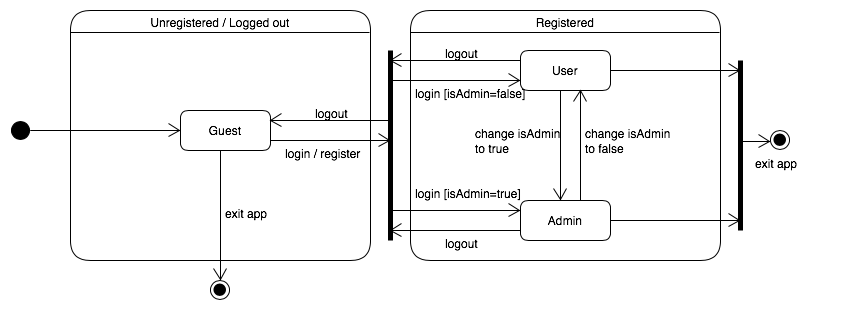
\includegraphics[width=0.8\textwidth]{User_Management/User_Management_State_Diagram.png}
\end{figure}

\subsection{Sequence Diagram}
\begin{figure}[!htbp]
	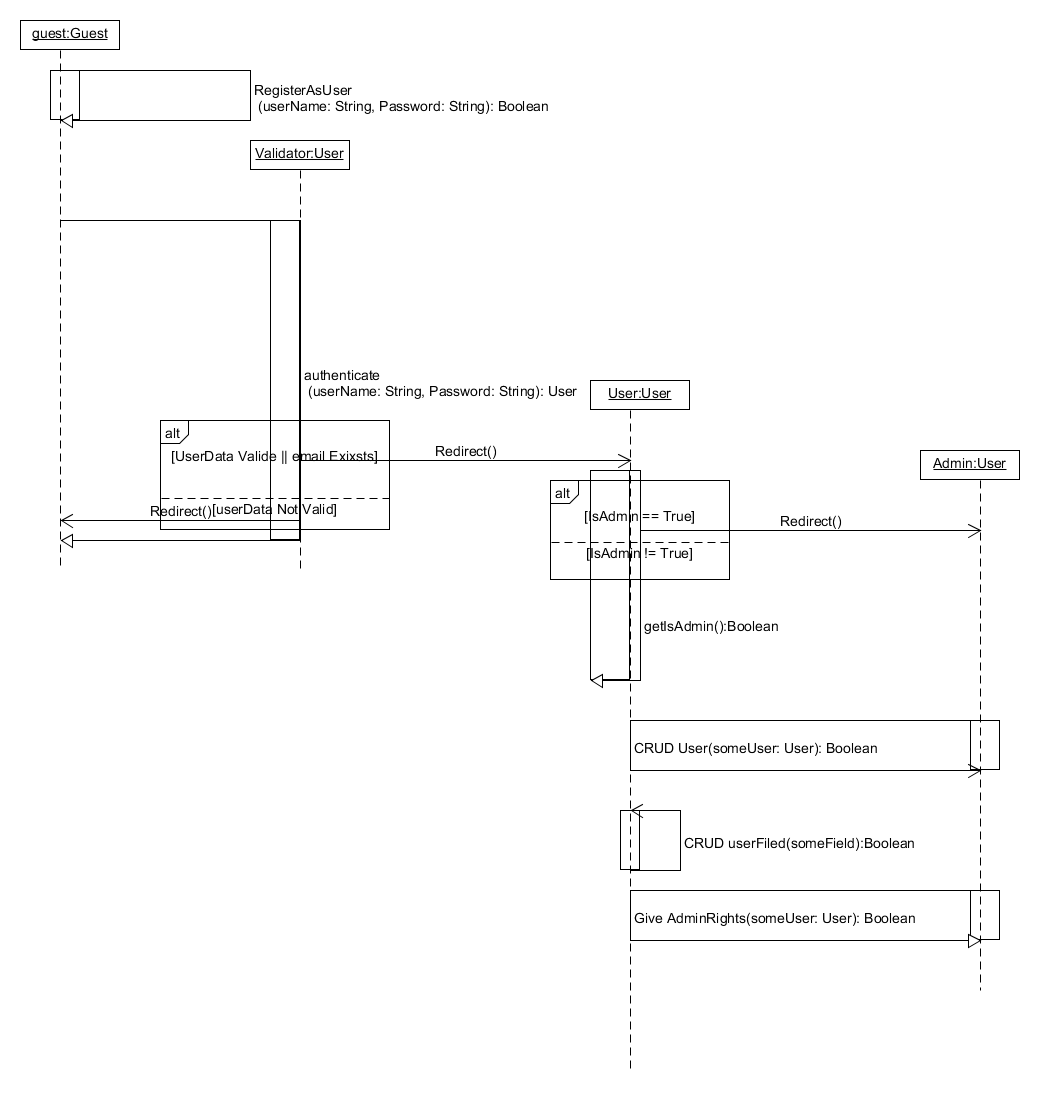
\includegraphics[width=0.8\textwidth]{User_Management/Sequence_Diagram_User_Management.png}
\end{figure}

\subsection{Package Diagram}

\subsection{Activity Diagram}
\begin{figure}[!htbp]
	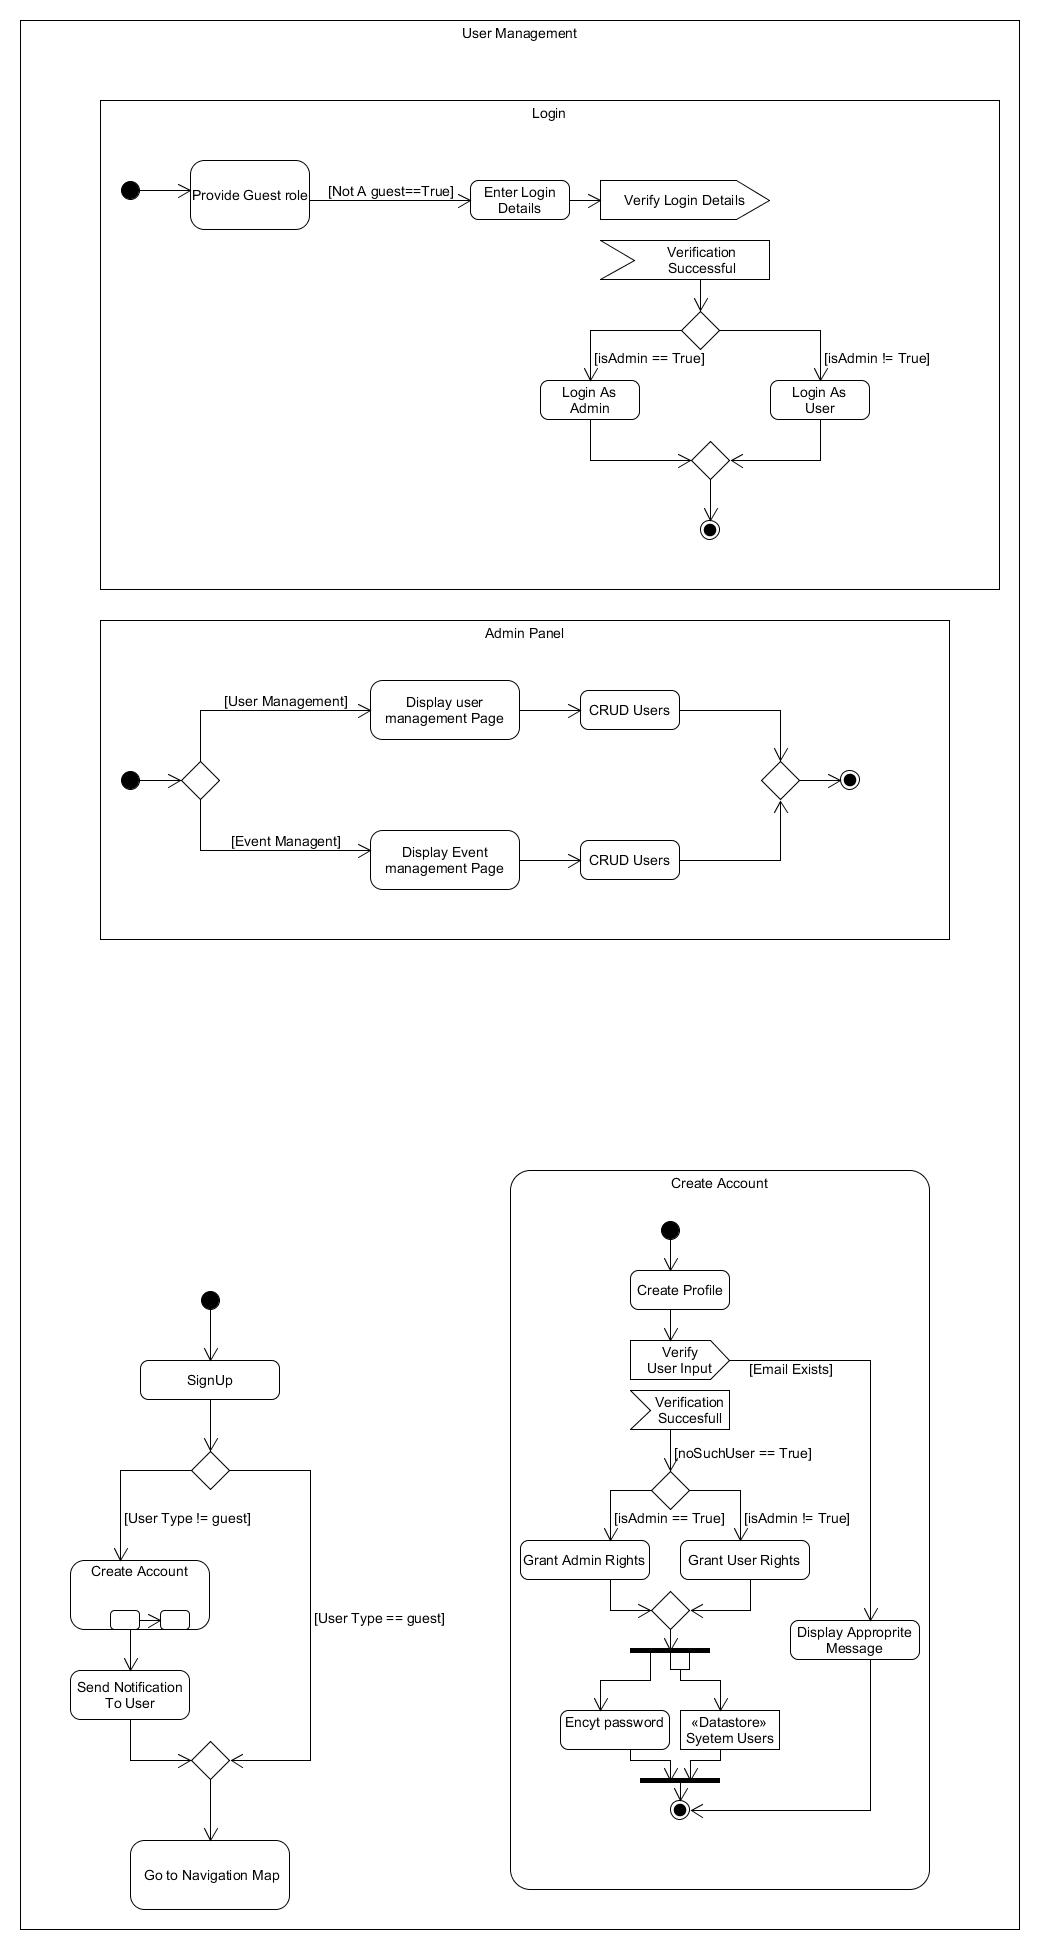
\includegraphics[width=0.8\textwidth]{User_Management/User_Management_Activity_Diagram.png}
\end{figure}
\clearpage

\subsection{Class Diagram}
\begin{figure}[!htbp]
	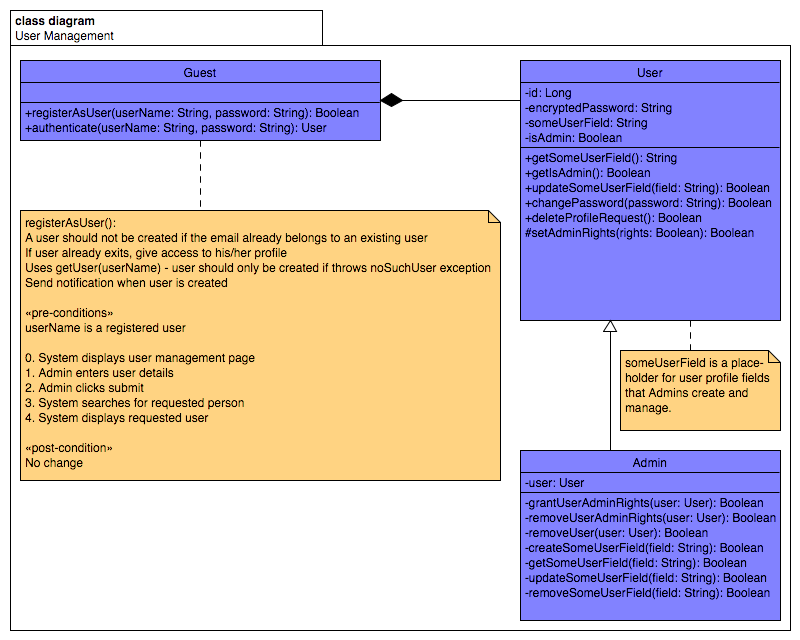
\includegraphics[width=\textwidth]{User_Management/User_Management_Class_Diagram.png}
\end{figure}

\clearpage

\section{Fitness}
	\subsection{Use Case Diagram}
\begin{figure}[!h]
  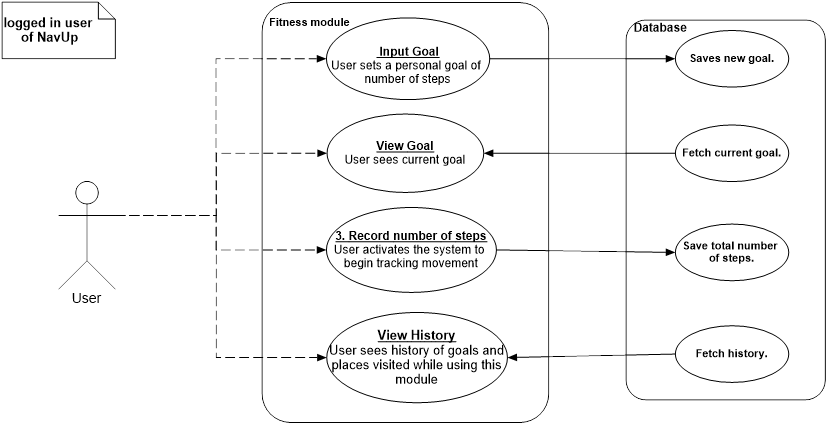
\includegraphics[width=0.8\textwidth]{Fitness/FitnessUseCase.png}
\end{figure}

\subsection{State Diagram}

\subsection{Sequence Diagram}

\subsection{Package Diagram}

\subsection{Activity Diagram}
\begin{figure}[!h]
  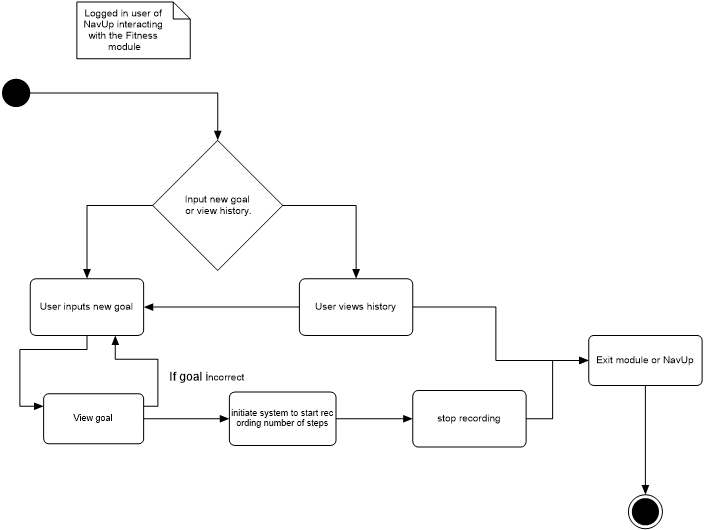
\includegraphics[width=0.8\textwidth]{Fitness/FitnessActivitydiagram.png}
\end{figure}

\subsection{Class Diagram}
\begin{figure}[!h]
  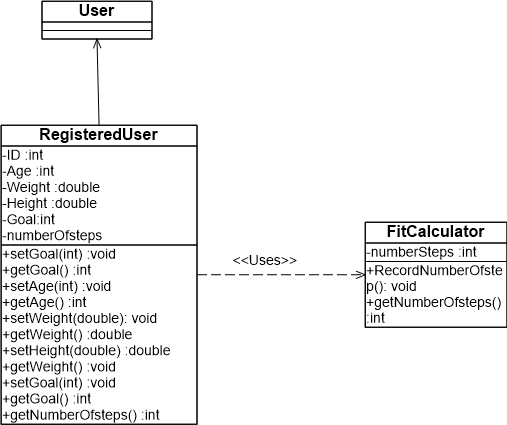
\includegraphics[width=0.8\textwidth]{Fitness/FitnessClassDgm.png}
\end{figure}

\end{document}
